\chapter{Results and Analysis}
\label{results}

This chapter details the results of tuning and evaluating the CGT model. For the genre model, only the drama category was used, as it was the most evenly balanced class.

\section{Hyperparameter grid search}
A number of grid searches were performed to tune the hyperparameters of the CGT model. Due to the different sizes of the MovieLens (ML) datasets, the smallest dataset, ML100k, was used to test the widest range of hyperparameters. Then, the set of hyperparameters used across the top performing models on ML100k were tested on the ML1M dataset. No hyperparameter tuning was done on ML10M due to its size. The best hyperparameters from ML1M were used for ML10M.

In each grid search, the best parameters were chosen as those which minimised the average CV log loss of the genre classifications.

When initialising weights of each model, the same random seed was used to allow for reproducible results.

\subsection{MovieLens100k}
Three grid searches were performed on the ML100k dataset. The first grid search tested various combinations of $k$ -- the number of latent factors, $h$ -- the number of hidden nodes in the rating model, and $j$ -- the number of hidden nodes in the genre model. The second grid search tested different numbers of training epochs and the third test different values of $dr1$ and $dr2$ -- the dropout rate in the hidden layers of each model. Finally, a number of different activation functions were tested. Each successive hyperparameter search used the best set of hyperparameters from the previous.

\subsubsection{Number of latent factors and hidden neurons}
Values between 50 and 200 were tested for $k$, while $h$ and $j$ were tested between the range of 25 and 100. While tuning these parameters, the dropout rate of the hidden layers, $dr1$ and $dr2$ were both fixed at 0.2 and ReLU was used as the activation function. A total of 12 different combinations were tested in this grid search, the top 5 models are shown in table \ref{tab:ml100k-grid-results1}.

\begin{table}[H]
\centering
\begin{tabular}{c | c | c | c | c}
\toprule
\textbf{$k$} & \textbf{$h$} & \textbf{$j$} & \textbf{Avg. CV log loss} & \textbf{Avg. CV acc.} \% \\
\midrule
200 & 100 & 100 & 0.6339 & 63.85 \\
\midrule
200 & 100 & 50 & 0.6362 & 63.52 \\
\midrule
100 & 100 & 100 & 0.6381 & 63.25 \\
\midrule
100 & 50 & 100 & 0.6385 & 62.66 \\
\midrule
200 & 50 & 100 & 0.6392 & 63.05 \\
\bottomrule
\end{tabular}
\caption[MovieLens 100K grid search results -- number of nodes]{Hyperparameters of best 5 models on MovieLens 100K dataset, with dropout of 0.2 and ReLU activation function.}
\label{tab:ml100k-grid-results1}
\end{table}

The best performing set of hyperparameters in the first grid search was $k=200$, $h=100$ and $j=100$. All of the top five used a latent factor vector size of either 100 or 200. All top three models had a value of 100 for $h$, while four of the top five had a value of 100 for $j$. The relationship between the size of $k$ and the average CV loss is shown in figure \ref{fig:5-latent-size}

\begin{figure}[H]
\centering
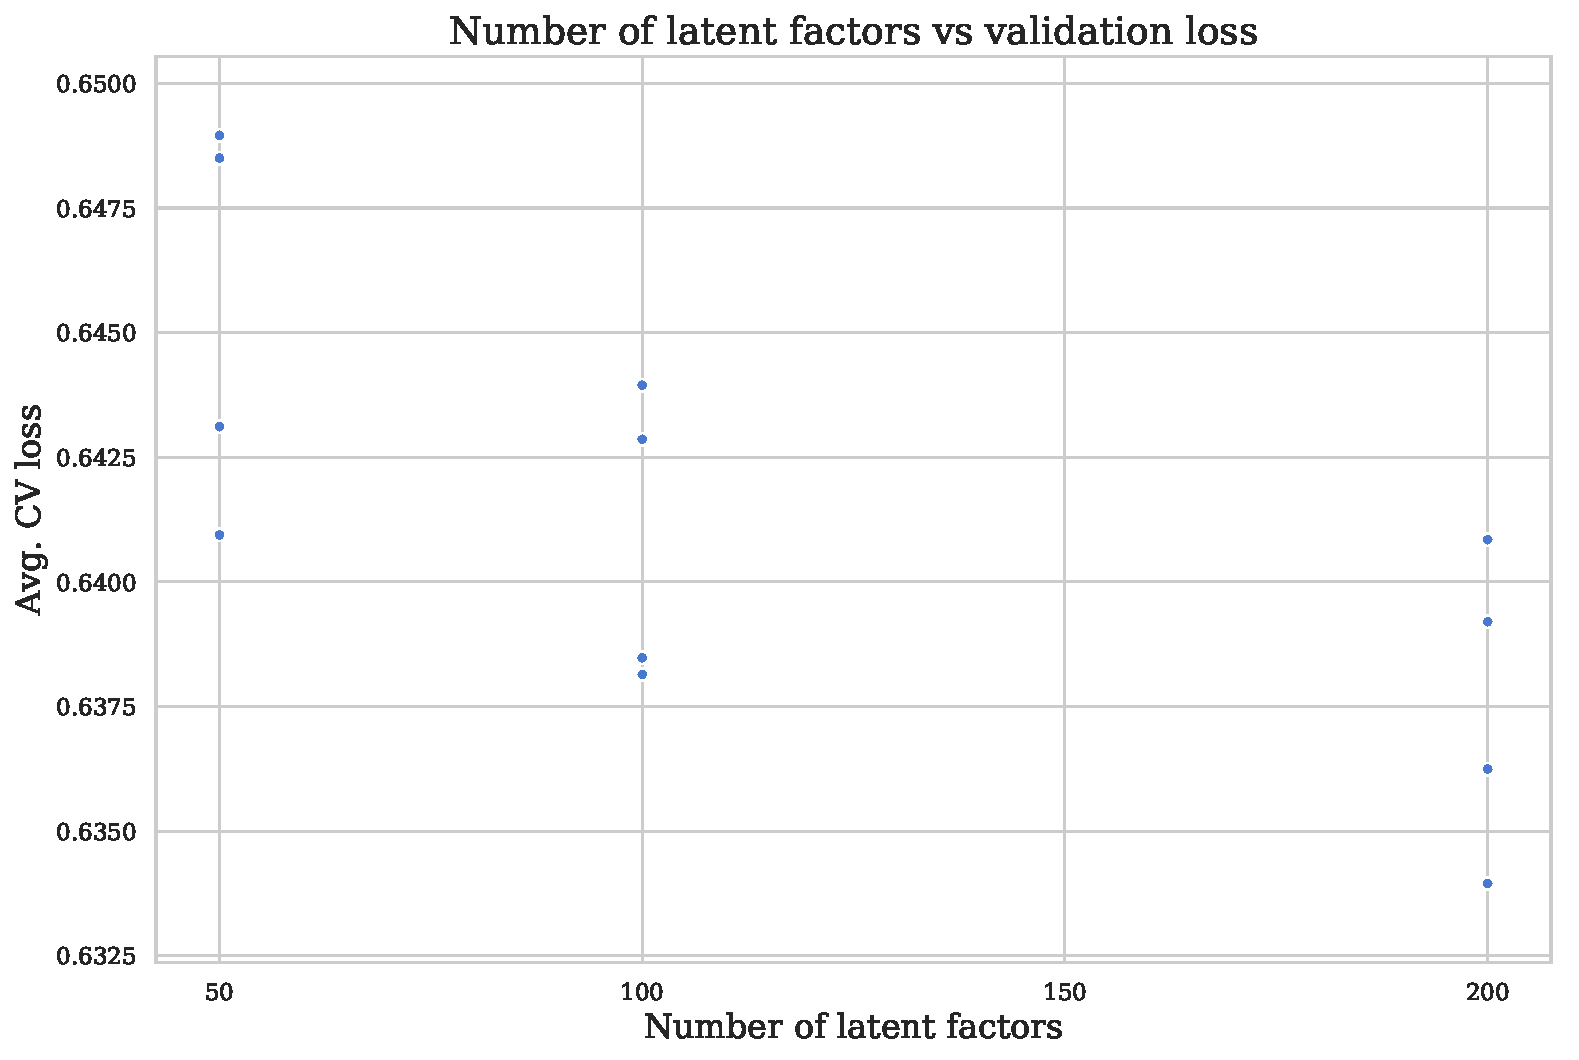
\includegraphics[width=0.8\textwidth]{Figures/5_ml100k-latent-factors.pdf}
\decoRule
\caption[Size of $k$]{Results of the first hyperparameter grid search. Size of $k$ is shown relative to the average CV loss for all 12 models.}
\label{fig:5-latent-size}
\end{figure}

\subsubsection{Number of epochs}
Training the model for too many epochs could risk overfitting. Therefore, it was necessary to find the optimal number of epochs for both the rating and genre model
A total of n different combinations were tested in this grid search, the top 5 models are shown in table \ref{tab:ml100k-grid-results2}.

\begin{table}[H]
\centering
\begin{tabular}{c | c | c | c}
\toprule
\textbf{$E1$} & \textbf{$E2$} & \textbf{Avg. CV log loss} & \textbf{Avg. CV acc.} \% \\
\midrule
7 & 5 & 0.6339 & 63.85 \\
\midrule
6 & 5 & 0.6346 & 63.65 \\
\midrule
7 & 4 & 0.6351 & 63.58 \\
\midrule
6 & 4 & 0.6355 & 62.65 \\
\midrule
5 & 5 & 0.6367 & 63.45 \\
\bottomrule
\end{tabular}
\caption[MovieLens 100K grid search results -- number of epochs]{Number of training epochs for both models.}
\label{tab:ml100k-grid-results2}
\end{table}

\subsubsection{Dropout rates}
The second grid search tested different combinations of dropout rates used in the hidden layers of the two models. Values between 0.15 and 0.25 were tested. A total of 9 different combinations were tested in this grid search, with each one using the hyperparameters $k$, $h$ and $j$ from the best performing model in the first grid search. The top 5 models from the second grid search are shown in table \ref{tab:ml100k-grid-results3}.

\begin{table}[H]
\centering
\begin{tabular}{c | c | c | c | c}
\toprule
\textbf{$dr1$} & \textbf{$dr2$} & \textbf{Avg. CV log loss} & \textbf{Avg. CV acc.} \% \\
\midrule
0.25 & 0.15 & 0.6334 & 63.05 \\
\midrule
0.25 & 0.2 & 0.6335 & 63.32 \\
\midrule
0.25 & 0.25 & 0.6337 & 63.19 \\
\midrule
0.2 & 0.15 & 0.6338 & 63.85 \\
\midrule
0.2 & 0.2 & 0.6339 & 63.85 \\
\bottomrule
\end{tabular}
\caption[MovieLens 100K grid search results -- dropout rates]{Best 5 dropout rates on MovieLens 100K dataset, with $k=200$, $h=100$, $j=100$}
\label{tab:ml100k-grid-results3}
\end{table}

\subsubsection{Activation function}
Finally, five different activation functions were tested using the best parameters from the first two grid searches. The five activation functions used were:
\begin{itemize}
    \item Linear
    \item Rectified Linear Unit (ReLU)
    \item Scaled Exponential Linear Unit (SELU)
    \item Softplus
    \item Hyperbolic tangent (Tanh)
\end{itemize}
The CV performance of each activation function is shown in \ref{tab:ml100k-activations}.

\begin{table}[H]
\centering
\begin{tabular}{c | c | c | c | c}
\toprule
\textbf{Activation function} & \textbf{Avg. CV log loss} & \textbf{Avg. CV acc.} \% \\
\midrule
ReLU & 0.6334 & 63.05 \\
\midrule
Softplus & 0.6430 & 61.40 \\
\midrule
SELU & 0.6441 & 61.92 \\
\midrule
Tanh & 0.6469 & 60.94 \\
\midrule
Linear & 0.6473 & 60.41 \\
\bottomrule
\end{tabular}
\caption[MovieLens 100K grid search results -- activation function]{Comparison of activation functions}
\label{tab:ml100k-activations}
\end{table}